\afterpage{%
\begin{figure}[p!]
	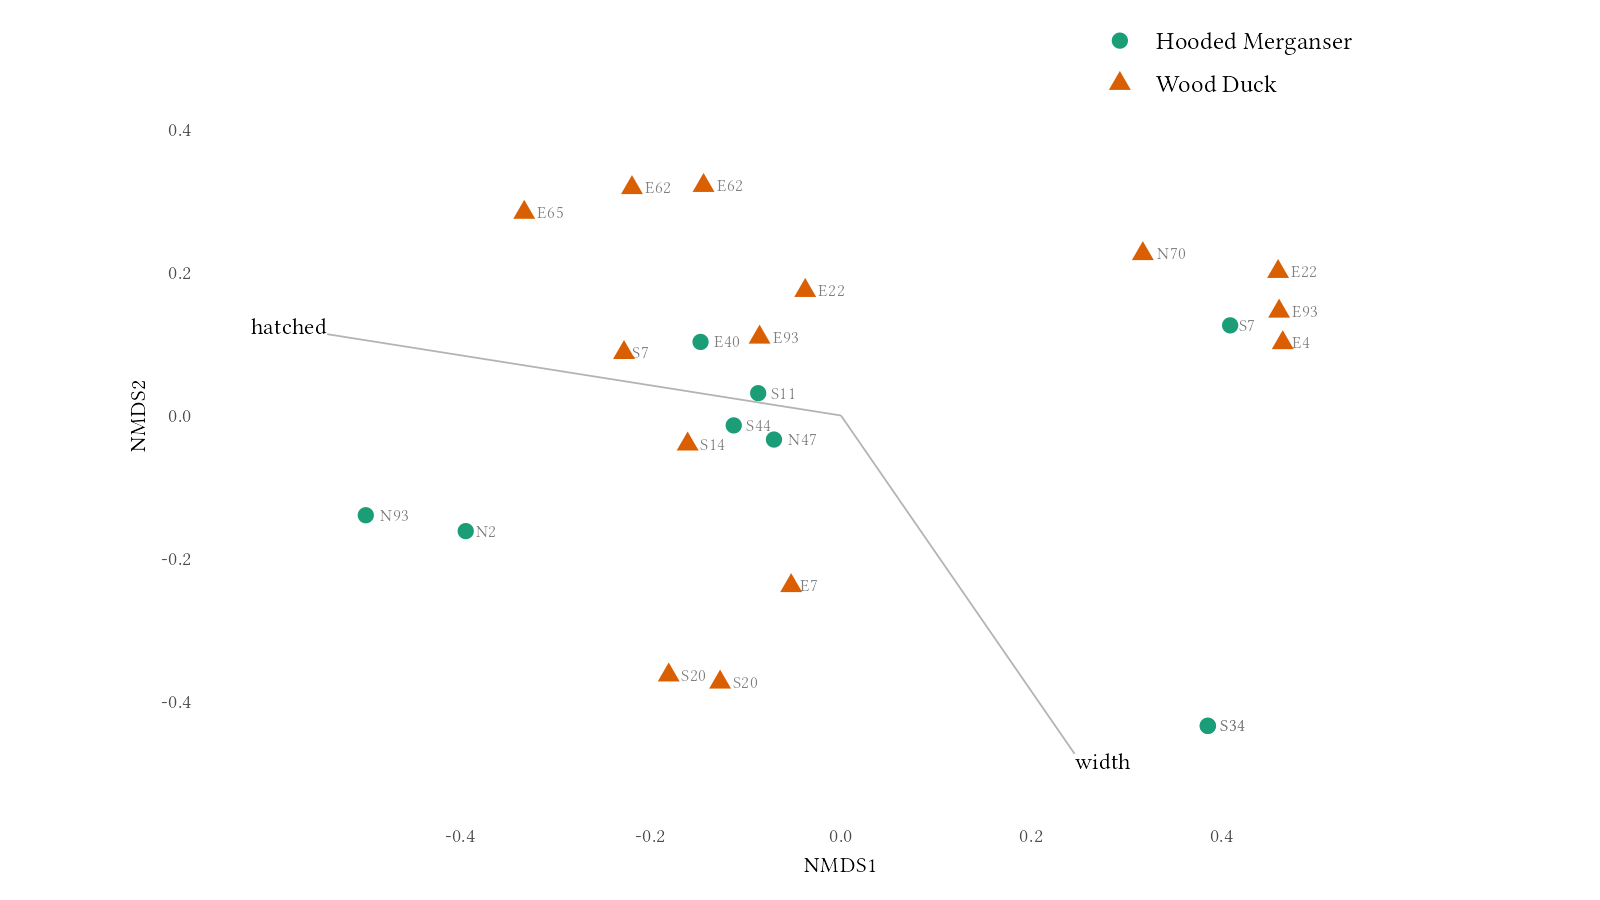
\includegraphics[width=\textwidth]{nmds_plot_axes12}
	\caption[N\textsc{mds} plot of axes 1 and 2]{Non-metric multidimensional analysis plot of axes 1 and 2. Green circles indicate nest boxes with Hooded Merganser as the original species. Orange triangles indicate nest boxes with Wood Duck as the original species. Light gray numbers show box~\textsc{id} numbers. N = Pool~1; E = Pool~2, S = Pool~3. Hatched and width variables provided the greatest rank-order separation on axis~1 and axis~2, respectively. Boxes to the left of the plot had greater numbers of hatched eggs. Boxes toward the lower half of the plot were associated with wider water. Stress = 0.023.}
	\label{fig:nmds_plot_axes12}
\end{figure}
\clearpage}
